\ifx\boi\undefined\ifx\problemname\undefined
\providecommand\sampleinputname{}
\providecommand\sampleoutputname{}
\documentclass[german]{templates/boi}
\problemlanguage{.de}
\fi
\newcommand{\boi}{Baltische Informatikolympiade}
\newcommand{\practicesession}{Practice Session}
\newcommand{\contestdates}{27. April - 1. Mai, 2018}
\newcommand{\dayone}{Tag 1}
\newcommand{\daytwo}{Tag 2}
\newcommand{\licensingtext}{Diese Aufgabenstellung ist unter der CC BY-SA 4.0 lizensiert.}
\newcommand{\problem}{Aufgabe}
\newcommand{\inputsection}{Eingabe}
\newcommand{\outputsection}{Ausgabe}
\newcommand{\interactivity}{Interaktivität}
\newcommand{\grading}{Grading}
\newcommand{\scoring}{Scoring}
\newcommand{\constraints}{Beschränkungen}
\renewcommand{\sampleinputname}{Beispieleingabe}
\renewcommand{\sampleoutputname}{Beispielausgabe}
\newcommand{\sampleexplanation}[1]{Beschreibung zu Beispiel #1}
\newcommand{\sampleexplanations}{Beschreibung der Beispiele}
\newcommand{\timelimit}{Zeitlimit}
\newcommand{\memorylimit}{Speicherlimit}
\newcommand{\seconds}{s}
\newcommand{\megabytes}{MB}
\newcommand{\group}{Gruppe}
\newcommand{\points}{Punkte}
\newcommand{\limitsname}{Limits}
\newcommand{\additionalconstraints}{Zusätzliche Beschränkungen}
\newcommand{\testgroups}{
Deine Lösung wird auf mehreren Testgruppen ausgeführt werden, von denen jede eine bestimmte Punktzahl wert ist.
Jede Testgruppe enthält mehrere Testcases. Um Punkte für eine Testgruppe zu bekommen, müssen alle Testfälle in der entsprechenden Gruppe gelöst werden.
Deine finale Punktzahl wird die maximal erreichte Punktzahl in allen Einsendungen sein.
}
\fi
\def\version{jury-1}
\problemname{Paths}
Ein {\em Graph} ist ein mathematisches Konstrukt das aus einer Menge an{\em Knoten} und einer Menge an {\em Kanten}, die jeweils mit zwei Knoten verbunden sind. Ein Beispiel eines Graphen mit $4$ Knoten und $3$ Kanten ist unten in der Erklärung des Beispiels abgebildet.

Ein {\em Pfad} ist definiert als geordnete Liste mit 2 oder mehr Knoten mit Kanten zwischen den aufeinanderfolgenden Knoten in der Liste. In dieser Aufgabe sind wir nur an {\em einfachen Pfaden} interessiert, in denen kein Knoten mehr als einmal vorkommt. Beachte, dass die Liste geordnet ist; z.B. ``\texttt{1-2-3}'', ``\texttt{1-3-2}'' und ``\texttt{3-2-1}'' sind unterschiedliche Pfade.

In dieser Aufgabe hat jeder Knoten im Graph eine von $K$ Farben. Die Aufgabe ist, die Anzahl der möglichen {\em (einfachen) Pfade} zu finden, in denen keine zwei Knoten die gleiche Farbe haben.


\section*{\inputsection}
Die erste Zeile des Inputs enthält drei Zahlen: $N$ (die Anzahl der Knoten), $M$ (die Anzahl der Kanten) und $K$ (die Anzahl der verschiedenen Farben).

Die zweite Zeile des Inputs enthält $N$ Zahlen zwischen $1$ und $K$ -- die Farben eines jeden Knotens (beginnend mit Knoten $1$ und endend mit Knoten $N$).

Jede der folgenden $M$ Zeilen beschreibt eine Kante und enthält zwei Nummern $a, b$ ($1 \le a, b \le N, a \neq b$) -- die zwei Knoten, die durch die Kante verbunden werden.

\section*{\outputsection}
Gib eine Zahl aus -- die Anzahl der Pfade, deren Knoten alle unterschiedliche Farben haben. Diese Anzahl wird immer kleiner als $10^{18}$ sein.

\section*{\constraints}
\testgroups

\noindent
\begin{tabular}{| l | l | l |}
\hline
\group & \points & \limitsname \\ \hline
1      & 23      & $1 \le N, M \le 100, 1 \le K \le 4$ \\ \hline
2      & 20      & $1 \le N, M \le 300\,000, 1 \le K \le 3$ \\ \hline
3      & 27      & $1 \le N, M \le 300\,000, 1 \le K \le 4$ \\ \hline
4      & 30      & $1 \le N, M \le 100\,000, 1 \le K \le 5$ \\ \hline
\end{tabular}

\section*{\sampleexplanation{1}}

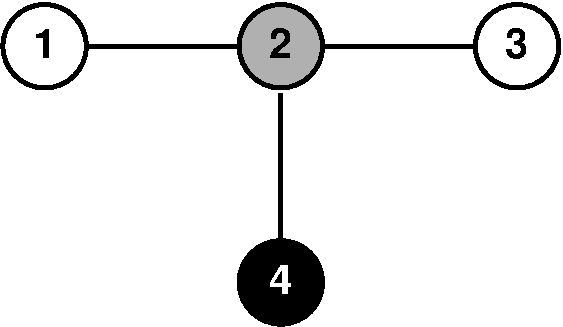
\includegraphics[width=5cm]{pathsfig.pdf}

Die Abbildung zeigt den Graph des ersten Beispiels, wobei jeder Knoten mit Weiß (Farbe 1), Grau (Farbe 2) oder Schwarz (Farbe 3) gefüllt ist. Es gibt 10 Pfade, deren Knoten alle unterschiedliche Farben haben: ``\texttt{1-2}'', ``\texttt{2-1}'', ``\texttt{2-3}'', ``\texttt{3-2}'', ``\texttt{2-4}'', ``\texttt{4-2}'', ``\texttt{1-2-4}'', ``\texttt{4-2-1}'', ``\texttt{3-2-4}'' und ``\texttt{4-2-3}''.

Beachte, dass weder ``\texttt{1}'' ein erlaubter Pfad ist, da es ein einzelner Knoten ist, noch ``\texttt{1-2-3}'', da er zwei Knoten der gleichen Farbe enthält.